\documentclass{beamer}
\usetheme[block = fill, titleformat title = allcaps, titleformat subtitle  = smallcaps,
progressbar = foot, background = light]{metropolis}           % Use metropolis theme
\usepackage{pgfplots}
\usepackage{fontawesome}
\usepackage{appendixnumberbeamer}
\usepackage{booktabs}
\usetikzlibrary{arrows.meta,positioning, shapes, backgrounds}

\usepackage[sortcites=false,style=authoryear-comp,bibencoding=utf8, natbib=true, firstinits=true, maxcitenames=2, maxbibnames = 99, uniquename=false, backend=bibtex, useprefix=true, backref=false,doi=false,isbn=false,url=false,dashed=true]{biblatex}
\setlength\bibhang{20pt}
\bibliography{../paper/references.bib}
\AtEveryBibitem{%
	\clearfield{day}%
	\clearfield{month}%
	\clearfield{endday}%
	\clearfield{endmonth}%
}
\AtBeginBibliography{\footnotesize}

\makeatletter
\let\save@measuring@true\measuring@true
\def\measuring@true{%
	\save@measuring@true
	\def\beamer@sortzero##1{\beamer@ifnextcharospec{\beamer@sortzeroread{##1}}{}}%
	\def\beamer@sortzeroread##1<##2>{}%
	\def\beamer@finalnospec{}%
}
\makeatother

\title{Housing market and migration revisited}
\subtitle{A Bayesian multilevel gravity model for Dutch municipalities}
\date{\today}
\author{Thomas de Graaff}
\institute{Vrije Universiteit Amsterdam\\Department of Spatial Economics}
\begin{document}
\maketitle

\begin{frame}{Background: two different cultures \citep{breiman2001statistical}}
	\begin{columns}
		\begin{column}{0.5\textwidth}
			In economics: 
			\begin{itemize}
				\item \alert{causal} impact of $x$ on $y$
				\item \alert{average} treatment effect
		    \end{itemize}
			\begin{center}
				
\includegraphics[width=0.5\textwidth]{../fig/harmless}      
			\end{center}
		\end{column}\pause
		\begin{column}{0.5\textwidth} 
		Outside economics: 
			\begin{itemize}
				\item \alert{model performance } 
				\item \alert{prediction} of total effect
			\end{itemize}
			\begin{center}
				
\includegraphics[width=0.5\textwidth]{../fig/rethinking}      
			\end{center}
		\end{column}
	\end{columns}
\end{frame}

  \begin{frame}{Background empirical application}
    	\begin{itemize}
		\item Aggregate homeownership has negative impact on labour market performance, because of increased \alert{moving costs} \citep{oswald1996conjecture,oswald1999housing}
		\newline
		\item Large empirical literature (mostly on individual decisions)
		\newline
		\item Literature on impact of social renting on migration flows is scarce \citep{de2009homeownership}
		\begin{itemize}
			\item Social renting rights only valid \alert{within} city \citep[but][]{boyle1998migration}
			\item Social renting is an \alert{urban} phenomenon ($\approx$ 40\% in Amsterdam)
		\end{itemize}
    	\end{itemize}
  \end{frame}

\begin{frame}{This paper}
	\begin{description}

		\item[Does what?] \alert{Revisits} the impact of housing market structure (homeownership and social renting) on within-country migration flows using a Bayesian multilevel gravity model \citep{congdon2010random}
		\newline
		\item[Aim] to be able to \alert{predict} all changes in incoming and outcoming migration flows of, e.g., Amsterdam, when housing market structure changes \alert{whilst} accounting for origin and destination specific effects \citep{ranjan2007bayesian}
	\end{description}
\end{frame}

\begin{frame}[fragile]{Gravity model data structure}
	 \begin{figure}	
   \begin{tikzpicture}[scale=0.90, thick]
   
   \tikzstyle{orig}=[rectangle, rounded corners, thin, fill=green!20, text=black, draw, minimum width=2.5cm]
   \tikzstyle{dest}=[rectangle, rounded corners, thin, fill=red!20, text=black, draw, minimum width=2.5cm]
   \tikzstyle{migrants}=[rectangle, rounded corners, thin, fill=blue!20, text=black, draw, minimum width=2.5cm]
   \tikzstyle{var}=[rectangle, rounded corners, thin, fill=black!10, text=black, draw, text width = 3.5cm]
   
   \node[orig] (o1) at (0,0)  {\textsc{Origin$_1$}};
   \node[orig] (o2) at (0,-1) {\textsc{Origin$_2$}};
   \node[orig] (o3) at (0,-2) {\textsc{Origin$_3$}};
   \node (o4) at (0,-3) {\textsc{\vdots}};
   \node[orig] (o5) at (0,-4) {\textsc{Origin$_i$}};
   \node (o6) at (0,-5) {\textsc{\vdots}};
   \node[orig] (o7) at (0,-6) {\textsc{Origin$_R$}};
   
   \node[dest] (d1) at (8,0)  {\textsc{Destination$_1$}};
   \node[dest] (d2) at (8,-1) {\textsc{Destination$_2$}};
   \node[dest] (d3) at (8,-2) {\textsc{Destination$_3$}};
   \node (d4) 		 at (8,-3) {\textsc{\vdots}};
   \node[dest] (d5) at (8,-4) {\textsc{Destination$_j$}};
   \node (d6) 		 at (8,-5) {\textsc{\vdots}};
   \node[dest] (d7) at (8,-6) {\textsc{Destination$_R$}};
%   
%   % Migratior links
%   \draw[-latex, blue, thin, dashed] (1.5,0) -- (6.5, 0);
%   \draw[-latex, blue, thin, dashed] (1.5,0) -- (6.5,-0.8);
%   \draw[-latex, blue, thin, dashed] (1.5,0) -- (6.5,-1.8);
%   \draw[-latex, blue, thin, dashed] (1.5,0) -- (6.5,-3.8);
%   \draw[-latex, blue, thin, dashed] (1.5,0) -- (6.5,-5.6);
%   
%   \draw[-latex, blue, thin, dashed] (1.5,-1) -- (6.5,-0.1);
%   \draw[-latex, blue, thin, dashed] (1.5,-1) -- (6.5,-0.9);
%   \draw[-latex, blue, thin, dashed] (1.5,-1) -- (6.5,-1.9);
%   \draw[-latex, blue, thin, dashed] (1.5,-1) -- (6.5,-3.9);
%   \draw[-latex, blue, thin, dashed] (1.5,-1) -- (6.5,-5.7);
%   
%   \draw[-latex, blue, thin, dashed] (1.5,-2) -- (6.5, -0.2);
%   \draw[-latex, blue, thin, dashed] (1.5,-2) -- (6.5,-1);
%   \draw[-latex, blue, thin, dashed] (1.5,-2) -- (6.5,-2);
%   \draw[-latex, blue, thin, dashed] (1.5,-2) -- (6.5,-4);
%   \draw[-latex, blue, thin, dashed] (1.5,-2) -- (6.5,-5.8);
%   
%   \draw[-latex, blue, thin, dashed] (1.5,-4) -- (6.5,-0.3);
%   \draw[-latex, blue, thin, dashed] (1.5,-4) -- (6.5,-1.1);
%   \draw[-latex, blue, thin, dashed] (1.5,-4) -- (6.5,-2.1);
%   \draw[-latex, blue, thin, dashed] (1.5,-4) -- (6.5,-4.1);
%   \draw[-latex, blue, thin, dashed] (1.5,-4) -- (6.5,-5.9);
%   
%   \draw[-latex, blue, thin, dashed] (1.5,-6) -- (6.5, -0.4);
%   \draw[-latex, blue, thin, dashed] (1.5,-6) -- (6.5,-1.2);
%   \draw[-latex, blue, thin, dashed] (1.5,-6) -- (6.5,-2.2);
%   \draw[-latex, blue, thin, dashed] (1.5,-6) -- (6.5,-4.2);
%   \draw[-latex, blue, thin, dashed] (1.5,-6) -- (6.5,-6);
%   
%   \node[migrants] (m) at (4,-3)  {\textsc{Flows $i \rightarrow j$}};
%   
%   \node[var] (v1) at (0,-8)  {\textsc{Origin-specific variables ($o_i, \mathbf{X_i}$)}};
%   \node[var] (v2) at (4,-8)  {\textsc{flow-specific variables ($\mathbf{X}_{ij}$) }};
%   \node[var] (v3) at (8,-8)  {\textsc{Destination-specific variables  ($d_j, \mathbf{X_j}$)}};
%   
%   \begin{pgfonlayer}{background}
%   \filldraw [line width=4mm,join=round,black!10]
%   (o1.north -| o1.west)  rectangle (o7.south -| o7.east)
%   (d1.north -| d1.west)  rectangle (d7.south -| d7.east);
%   \end{pgfonlayer}
%   
%   \draw[-latex, thick, black] (v1) -- (0,-6.5);
%   \draw[-latex, thick, black] (v2) -- (4,-6.5);
%   \draw[-latex, thick, black] (v3) -- (8,-6.5);
   \end{tikzpicture}
	\end{figure}
\end{frame}

\begin{frame}[fragile]{Gravity model data structure}
	\begin{figure}	
		\begin{tikzpicture}[scale=0.90, thick]
		
		\tikzstyle{orig}=[rectangle, rounded corners, thin, fill=green!20, text=black, draw, minimum width=2.5cm]
		\tikzstyle{dest}=[rectangle, rounded corners, thin, fill=red!20, text=black, draw, minimum width=2.5cm]
		\tikzstyle{migrants}=[rectangle, rounded corners, thin, fill=blue!20, text=black, draw, minimum width=2.5cm]
		\tikzstyle{var}=[rectangle, rounded corners, thin, fill=black!10, text=black, draw, minimum width = 2.5cm]
		
		\node[orig] (o1) at (0,0)  {\textsc{Origin$_1$}};
		\node[orig] (o2) at (0,-1) {\textsc{Origin$_2$}};
		\node[orig] (o3) at (0,-2) {\textsc{Origin$_3$}};
		\node (o4) at (0,-3) {\textsc{\vdots}};
		\node[orig] (o5) at (0,-4) {\textsc{Origin$_i$}};
		\node (o6) at (0,-5) {\textsc{\vdots}};
		\node[orig] (o7) at (0,-6) {\textsc{Origin$_R$}};
		
		\node[dest] (d1) at (8,0)  {\textsc{Destination$_1$}};
		\node[dest] (d2) at (8,-1) {\textsc{Destination$_2$}};
		\node[dest] (d3) at (8,-2) {\textsc{Destination$_3$}};
		\node (d4) 		 at (8,-3) {\textsc{\vdots}};
		\node[dest] (d5) at (8,-4) {\textsc{Destination$_j$}};
		\node (d6) 		 at (8,-5) {\textsc{\vdots}};
		\node[dest] (d7) at (8,-6) {\textsc{Destination$_R$}};
		   
		   % Migratior links
		   \draw[-latex, blue, thin, dashed] (1.5,0) -- (6.5, 0);
		   \draw[-latex, blue, thin, dashed] (1.5,0) -- (6.5,-0.8);
		   \draw[-latex, blue, thin, dashed] (1.5,0) -- (6.5,-1.8);
		   \draw[-latex, blue, thin, dashed] (1.5,0) -- (6.5,-3.8);
		   \draw[-latex, blue, thin, dashed] (1.5,0) -- (6.5,-5.6);
		   
		   \draw[-latex, blue, thin, dashed] (1.5,-1) -- (6.5,-0.1);
		   \draw[-latex, blue, thin, dashed] (1.5,-1) -- (6.5,-0.9);
		   \draw[-latex, blue, thin, dashed] (1.5,-1) -- (6.5,-1.9);
		   \draw[-latex, blue, thin, dashed] (1.5,-1) -- (6.5,-3.9);
		   \draw[-latex, blue, thin, dashed] (1.5,-1) -- (6.5,-5.7);
		   
		   \draw[-latex, blue, thin, dashed] (1.5,-2) -- (6.5, -0.2);
		   \draw[-latex, blue, thin, dashed] (1.5,-2) -- (6.5,-1);
		   \draw[-latex, blue, thin, dashed] (1.5,-2) -- (6.5,-2);
		   \draw[-latex, blue, thin, dashed] (1.5,-2) -- (6.5,-4);
		   \draw[-latex, blue, thin, dashed] (1.5,-2) -- (6.5,-5.8);
		   
		   \draw[-latex, blue, thin, dashed] (1.5,-4) -- (6.5,-0.3);
		   \draw[-latex, blue, thin, dashed] (1.5,-4) -- (6.5,-1.1);
		   \draw[-latex, blue, thin, dashed] (1.5,-4) -- (6.5,-2.1);
		   \draw[-latex, blue, thin, dashed] (1.5,-4) -- (6.5,-4.1);
		   \draw[-latex, blue, thin, dashed] (1.5,-4) -- (6.5,-5.9);
		   
		   \draw[-latex, blue, thin, dashed] (1.5,-6) -- (6.5, -0.4);
		   \draw[-latex, blue, thin, dashed] (1.5,-6) -- (6.5,-1.2);
		   \draw[-latex, blue, thin, dashed] (1.5,-6) -- (6.5,-2.2);
		   \draw[-latex, blue, thin, dashed] (1.5,-6) -- (6.5,-4.2);
		   \draw[-latex, blue, thin, dashed] (1.5,-6) -- (6.5,-6);
		   
		   \node[migrants] (m) at (4,-3)  {\textsc{Flows $i \rightarrow j$}};
		   
		%   \node[var] (v1) at (0,-8)  {\textsc{Origin-specific variables ($o_i, \mathbf{X_i}$)}};
		   \node[var] (v2) at (4,-8)  {\textsc{Flow ($\mathbf{X}_{ij}$) }};
		%   \node[var] (v3) at (8,-8)  {\textsc{Destination-specific variables  ($d_j, \mathbf{X_j}$)}};
		%   
		%   \begin{pgfonlayer}{background}
		%   \filldraw [line width=4mm,join=round,black!10]
		%   (o1.north -| o1.west)  rectangle (o7.south -| o7.east)
		%   (d1.north -| d1.west)  rectangle (d7.south -| d7.east);
		%   \end{pgfonlayer}
		%   
		%   \draw[-latex, thick, black] (v1) -- (0,-6.5);
		   \draw[-latex, thick, black] (v2) -- (4,-6.5);
		%   \draw[-latex, thick, black] (v3) -- (8,-6.5);
		\end{tikzpicture}
	\end{figure}
\end{frame}

\begin{frame}[fragile]{Gravity model data structure}
	\begin{figure}	
		\begin{tikzpicture}[scale=0.90, thick]
		
		\tikzstyle{orig}=[rectangle, rounded corners, thin, fill=green!20, text=black, draw, minimum width=2.5cm]
		\tikzstyle{dest}=[rectangle, rounded corners, thin, fill=red!20, text=black, draw, minimum width=2.5cm]
		\tikzstyle{migrants}=[rectangle, rounded corners, thin, fill=blue!20, text=black, draw, minimum width=2.5cm]
		\tikzstyle{var}=[rectangle, rounded corners, thin, fill=black!10, text=black, draw, minimum width = 2.5cm]
		
		\node[orig] (o1) at (0,0)  {\textsc{Origin$_1$}};
		\node[orig] (o2) at (0,-1) {\textsc{Origin$_2$}};
		\node[orig] (o3) at (0,-2) {\textsc{Origin$_3$}};
		\node (o4) at (0,-3) {\textsc{\vdots}};
		\node[orig] (o5) at (0,-4) {\textsc{Origin$_i$}};
		\node (o6) at (0,-5) {\textsc{\vdots}};
		\node[orig] (o7) at (0,-6) {\textsc{Origin$_R$}};
		
		\node[dest] (d1) at (8,0)  {\textsc{Destination$_1$}};
		\node[dest] (d2) at (8,-1) {\textsc{Destination$_2$}};
		\node[dest] (d3) at (8,-2) {\textsc{Destination$_3$}};
		\node (d4) 		 at (8,-3) {\textsc{\vdots}};
		\node[dest] (d5) at (8,-4) {\textsc{Destination$_j$}};
		\node (d6) 		 at (8,-5) {\textsc{\vdots}};
		\node[dest] (d7) at (8,-6) {\textsc{Destination$_R$}};
		
		% Migratior links
		\draw[-latex, blue, thin, dashed] (1.5,0) -- (6.5, 0);
		\draw[-latex, blue, thin, dashed] (1.5,0) -- (6.5,-0.8);
		\draw[-latex, blue, thin, dashed] (1.5,0) -- (6.5,-1.8);
		\draw[-latex, blue, thin, dashed] (1.5,0) -- (6.5,-3.8);
		\draw[-latex, blue, thin, dashed] (1.5,0) -- (6.5,-5.6);
		
		\draw[-latex, blue, thin, dashed] (1.5,-1) -- (6.5,-0.1);
		\draw[-latex, blue, thin, dashed] (1.5,-1) -- (6.5,-0.9);
		\draw[-latex, blue, thin, dashed] (1.5,-1) -- (6.5,-1.9);
		\draw[-latex, blue, thin, dashed] (1.5,-1) -- (6.5,-3.9);
		\draw[-latex, blue, thin, dashed] (1.5,-1) -- (6.5,-5.7);
		
		\draw[-latex, blue, thin, dashed] (1.5,-2) -- (6.5, -0.2);
		\draw[-latex, blue, thin, dashed] (1.5,-2) -- (6.5,-1);
		\draw[-latex, blue, thin, dashed] (1.5,-2) -- (6.5,-2);
		\draw[-latex, blue, thin, dashed] (1.5,-2) -- (6.5,-4);
		\draw[-latex, blue, thin, dashed] (1.5,-2) -- (6.5,-5.8);
		
		\draw[-latex, blue, thin, dashed] (1.5,-4) -- (6.5,-0.3);
		\draw[-latex, blue, thin, dashed] (1.5,-4) -- (6.5,-1.1);
		\draw[-latex, blue, thin, dashed] (1.5,-4) -- (6.5,-2.1);
		\draw[-latex, blue, thin, dashed] (1.5,-4) -- (6.5,-4.1);
		\draw[-latex, blue, thin, dashed] (1.5,-4) -- (6.5,-5.9);
		
		\draw[-latex, blue, thin, dashed] (1.5,-6) -- (6.5, -0.4);
		\draw[-latex, blue, thin, dashed] (1.5,-6) -- (6.5,-1.2);
		\draw[-latex, blue, thin, dashed] (1.5,-6) -- (6.5,-2.2);
		\draw[-latex, blue, thin, dashed] (1.5,-6) -- (6.5,-4.2);
		\draw[-latex, blue, thin, dashed] (1.5,-6) -- (6.5,-6);
		
		\node[migrants] (m) at (4,-3)  {\textsc{Flows $i \rightarrow j$}};
		
		\node[var] (v1) at (0,-8)  {\textsc{Origin  ($o_i, \mathbf{X_i}$)}};
		\node[var] (v2) at (4,-8)  {\textsc{Flow ($\mathbf{X}_{ij}$) }};
		   \node[var] (v3) at (8,-8)  {\textsc{Destination ($d_j, \mathbf{X_j}$)}};
		   
		   \begin{pgfonlayer}{background}
		   \filldraw [line width=4mm,join=round,black!10]
		   (o1.north -| o1.west)  rectangle (o7.south -| o7.east)
		   (d1.north -| d1.west)  rectangle (d7.south -| d7.east);
		   \end{pgfonlayer}
		   
		   \draw[-latex, thick, black] (v1) -- (0,-6.5);
		\draw[-latex, thick, black] (v2) -- (4,-6.5);
		   \draw[-latex, thick, black] (v3) -- (8,-6.5);
		\end{tikzpicture}
	\end{figure}
\end{frame}

\begin{frame}{Why a Bayesian multilevel approach?}
\begin{itemize}
	\item Frequently used---increases model \alert{performance} and \alert{flexibility} 
    \item \alert{Simultenous} modeling at various levels (e.g., cities, regions, flows, individuals) 
    \begin{itemize}
    	\item No two-stage models anymore
    \end{itemize}
    \item Many definitions (in a Bayesian context):
	    \begin{itemize}
	    \item mixed effects, varying intercepts/parameter, shrinkage, partial pooling
	    \end{itemize}
	\item \alert{Estimates} the level effects from a distribution, usually $\sim \text{ Normal}(\alpha, \sigma)$
	\begin{itemize}
		\item $\sigma \longrightarrow 0$ : complete pooling
		\item $\sigma \longrightarrow \infty$ : no pooling (fixed effects)
	\end{itemize}
\end{itemize}
\end{frame}

\begin{frame}{Data: migrations flows}
	\begin{center}
		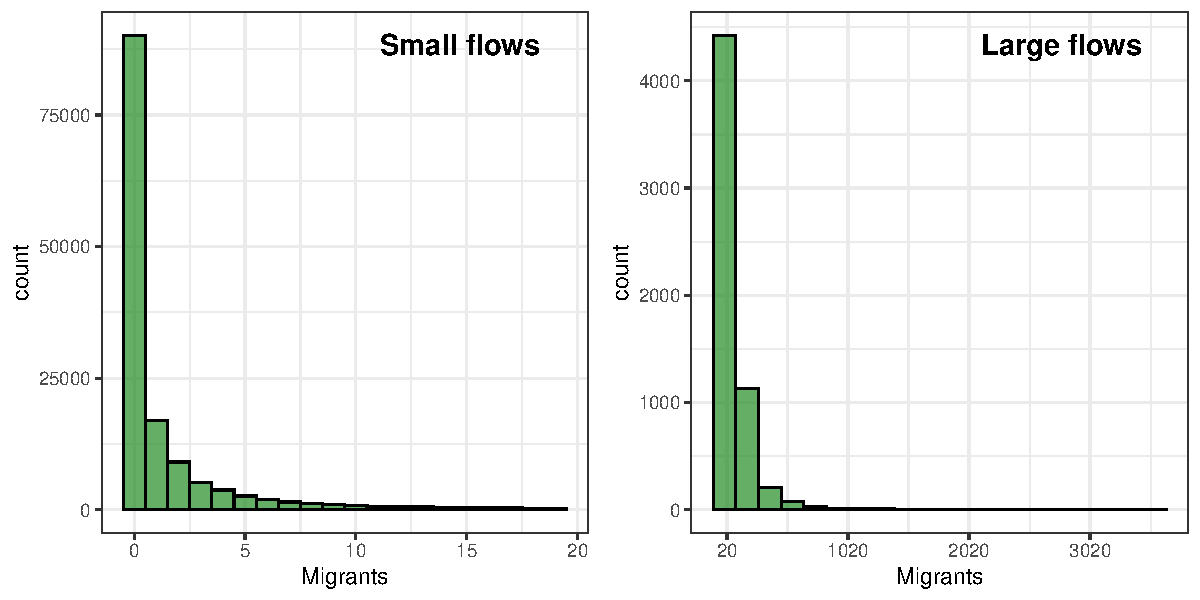
\includegraphics[width=0.8\textwidth]{../fig/hist_mig}      
	\end{center}
\begin{itemize}
	\item Individual migrations flows \alert{between} 393 Dutch cities in 2015
	\item Variance is 4 times expectation (dispersion)
\end{itemize}
\end{frame}

\begin{frame}{Data: municipal housing structure}
\begin{center}
	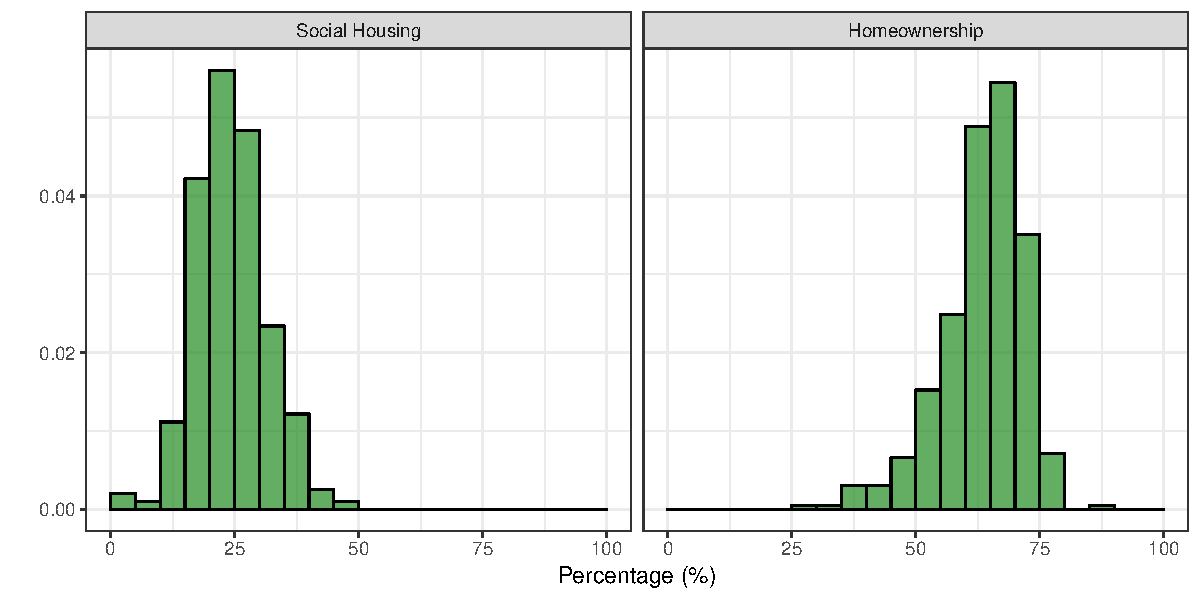
\includegraphics[width=0.8\textwidth]{../fig/hist_housing}      
\end{center}
\begin{itemize}
	\item Positive correlation between city size and social renting ($0.4$)
	\item Negative correlation between social renting and homeownership ($-0.84)$
\end{itemize}
\end{frame}

\begin{frame}{Modeling framework: traditional gravity modeling}
	\begin{equation*}
	\log(\text{migrants}_{ij}) = o_i + d_j +  \gamma\log(\text{dist}_{ij}) + \epsilon_{ij}
	\label{eq:gravfixed}
	\end{equation*} 
	
	Adopting fixed effects for multilateral resistance \citep{anderson2003gravity}, but
	\begin{itemize}
		\item what about zeros?
		\item how to incorporate municipal housing structure?
		\item dispersion and heteroskedasticity \citep{silva2006log}
	\end{itemize}
\end{frame}

\begin{frame}[fragile]{Modeling framework: multilevel gravity modeling}
\begin{small}
	\begin{align} \text{Migrants}_{ij} \sim & \text{ GammaPoisson}(\lambda_{ij}, \tau) \tag{\footnotesize \color{blue} outcome variable} \\ \pause
	\log(\lambda_{ij}) =
	& \alpha + o_{\text{mun}[i]} + d_{\text{mun}[j]} + \notag
	\\ & \beta_1 \log(\text{pop}_i) + \notag
	\beta_2\log(\text{pop}_j) + \notag \\ & \beta_3
	\log(\text{home}_i) + \beta_4 \log(\text{home}_j) + \notag\\
	& \beta_5 \log(\text{soc}_i) + \beta_6 \log(\text{soc}_j) + \notag \\ 
	& \beta_7 \log(\text{dist}_{ij})  \tag{\footnotesize \color{blue} linear model}  \\ \pause
	o_{\text{mun}} \sim& \text{ Normal}(\alpha_o, \sigma_o)  \tag{\footnotesize \color{blue} origin effects}  \\ 
	d_{\text{mun}} \sim& \text{ Normal}(\alpha_d, \sigma_d)   \tag{\footnotesize \color{blue} destination effects}  \\ \pause
	\beta_1,\ldots, \beta_7,\alpha_o, \alpha_d \sim& \text{
		Normal}(0,2) \tag{\footnotesize \color{blue} priors} \\ 
	\alpha_o, \alpha_d \sim& \text{ Normal}(0,2) \tag{\footnotesize \color{blue} priors}  \\
	\sigma_o, \sigma_d \sim& \text{ HalfCauchy}(0,1) \tag{\footnotesize \color{blue} priors}  \\ 
	\tau \sim& \text{ Gamma}(0.01, 0.01)  \tag{\footnotesize \color{blue} prior}  
	\end{align}
\end{small}
\end{frame}

\begin{frame}{Hamiltonian Monte Carlo (HMC) estimation results}
		\begin{columns}
		\begin{column}{0.5\textwidth}
			\begin{center}
				\begin{footnotesize}
			  \begin{tabular}{lrr}
				\toprule
				Parameter & mean & sd \\ 
				\midrule
				Intercept      & $-0.74$ & 0.04 \\ 
				log(pop$_i$)   & 0.89 & 0.03  \\ 
				log(pop$_j$)   & 0.88 & 0.04  \\ 
				log(home$_i$)  & $-1.48$ & 0.19 \\ 
				log(home$_j$)  & $-1.27$ & 0.25  \\ 
				log(soc$_i$)   & $-0.04$ & 0.04  \\
				log(soc$_j$)   & $-0.06$ & 0.03 \\ 
				log(dist$_{ij})$ & $-1.96$ & 0.01  \\ 
				$\sigma_o$    & 0.45 & 0.02  \\ 
				$\sigma_j$    & 0.61 & 0.02  \\ 
				$\tau$        & 1.22 & 0.01  \\ 
				\bottomrule
			\end{tabular}
		\end{footnotesize}
		\end{center}
		\end{column}
		\begin{column}{0.5\textwidth} 

			\begin{center}
				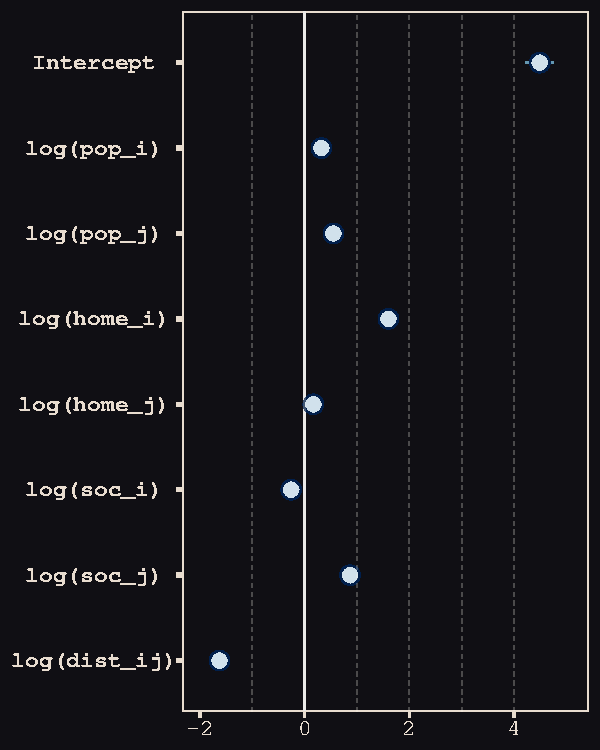
\includegraphics[width=\textwidth]{../fig/forestplot}      
			\end{center}
		\end{column}
	\end{columns}
\end{frame}

\begin{frame}{$d_{\text{mun}}$ as measure of attractivity?}
		\begin{columns}
	\begin{column}{0.5\textwidth}
		\begin{center}
			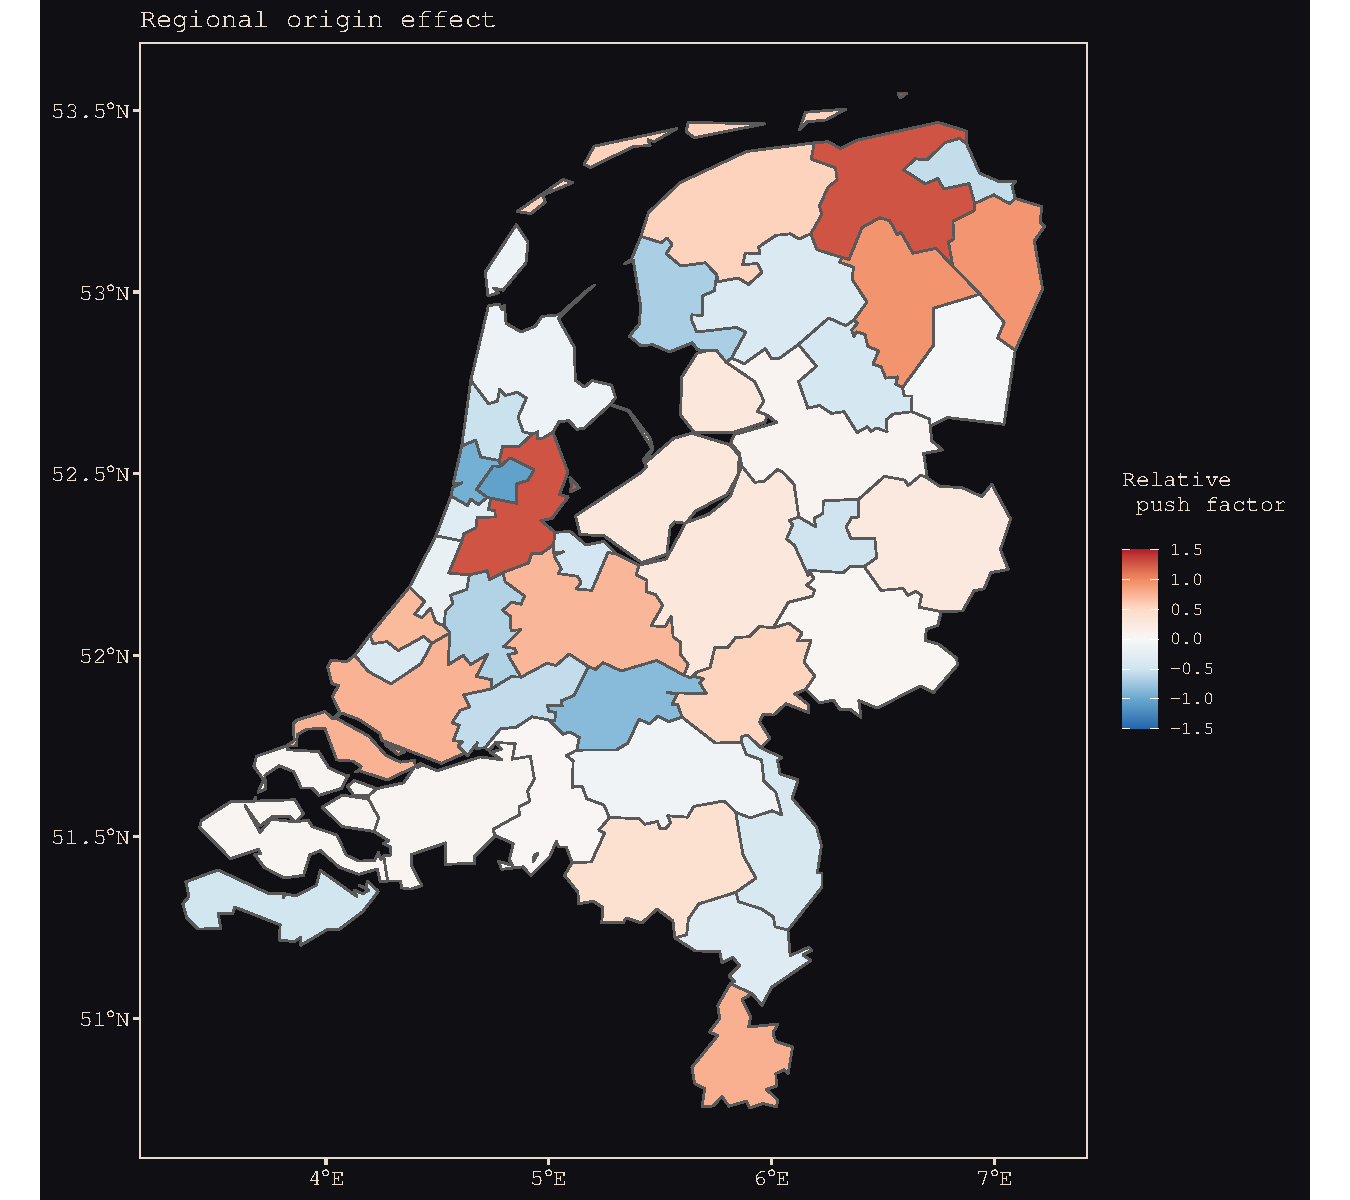
\includegraphics[width=1.1\textwidth]{../fig/p_coef_out}      
		\end{center}
	\end{column}\pause
	\begin{column}{0.5\textwidth} 	
		\begin{center}
			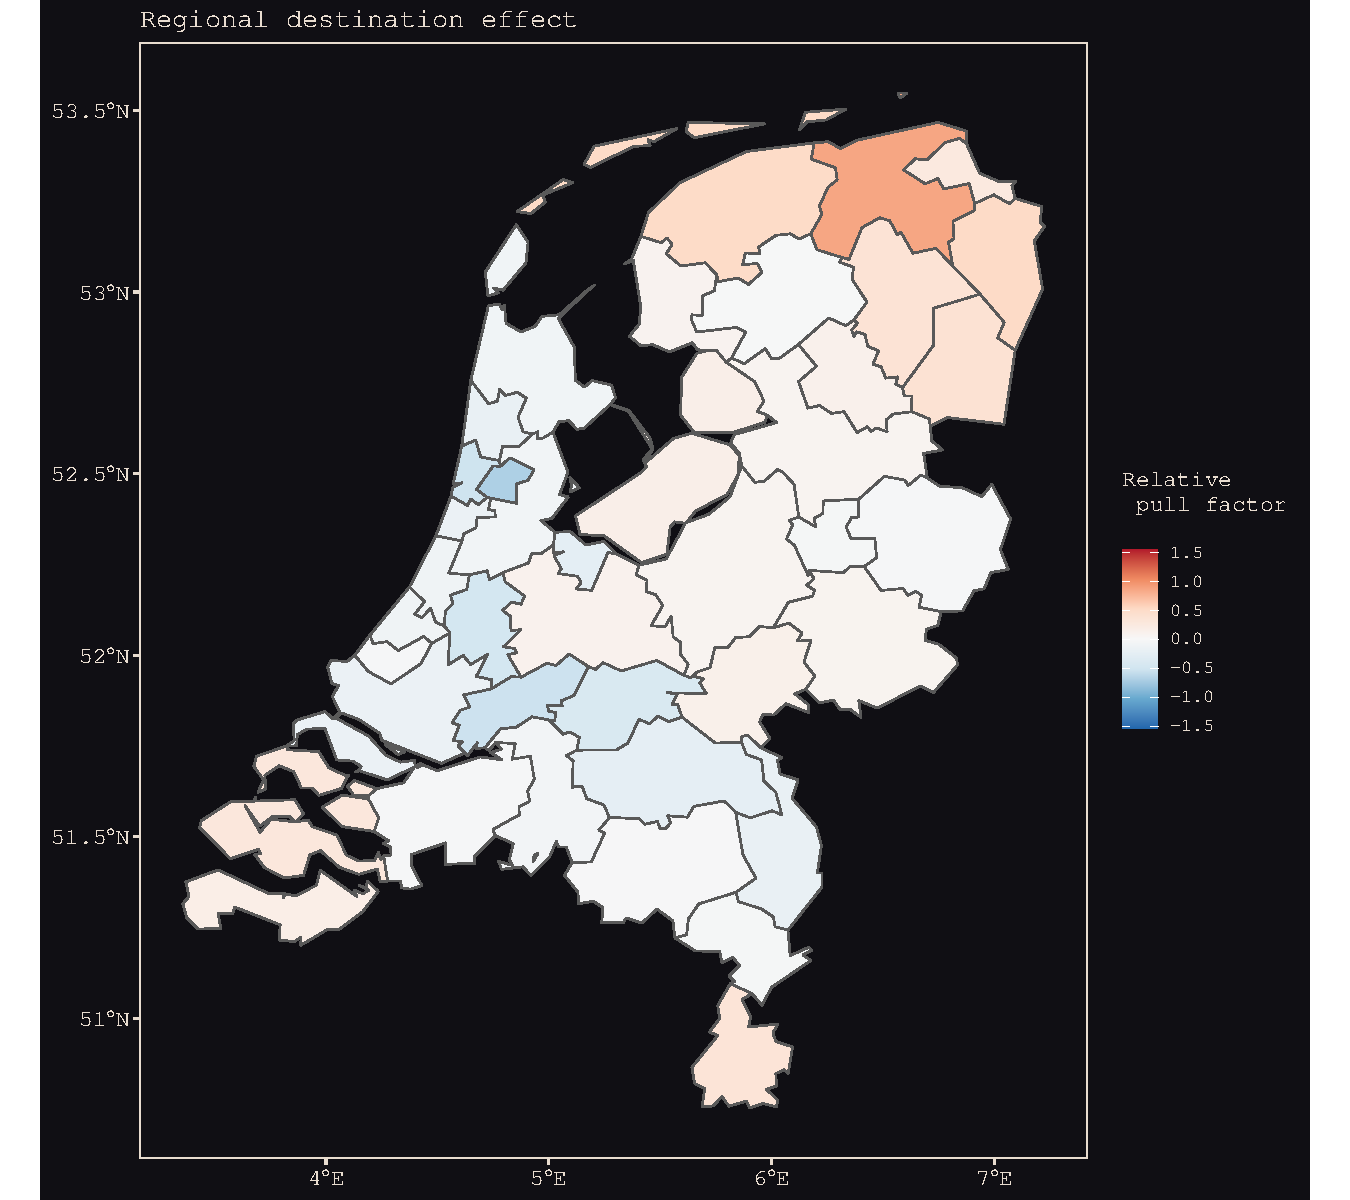
\includegraphics[width=1.1\textwidth]{../fig/p_coef_in}      
		\end{center}
	\end{column}
\end{columns}
\end{frame}

\begin{frame}{Predictions}
content...
\end{frame}

\begin{frame}{Conclusions}
With respect to migration flows:
\begin{itemize}
	\item homeownership has an elasticity well below $-1$
	\item social renting has negative elasticity as well, but close to zero
	\item most migration dynamics outside the most popular areas 
\end{itemize}

Multilevel gravity framework
\begin{itemize}
	\item flexible and powerful
	\item suitable for predictions \alert{within} and \alert{outside} sample
	\item with good model specification, estimation runs smoothly
	\item not very scalable; 154,056 obs. $\approx$ 6 hrs. of estimation
\end{itemize}
\end{frame}

\begin{frame}{Supplementary materials}

Paper, data and code can be retrieved from the project's GitHub page: 

\begin{center}\url{https://github.com/Thdegraaff/migration\_gravity}\end{center}

\faGithub\  \faCreativeCommons

\end{frame}

\begin{frame}[standout]
Questions?
\end{frame}

\appendix

\begin{frame}[allowframebreaks]{References}

		\printbibliography[heading=none]

\end{frame}


\end{document}